\section{ネットワーク設計}

\subsection{ネットワーク構成}
本システムにおけるネットワーク構成を図\ref{fig:network_design}に示す。
本システムは、インターネットを経由して接続される参加者端末および主催者端末と、
クラウド上に構築されたWeb/APサーバおよびデータベースによって構成される。

各端末はWebブラウザを介してシステムへアクセスする構成とし、
スマートフォンおよびPCの双方からの操作に対応している。

\begin{figure}[H]
    \centering
    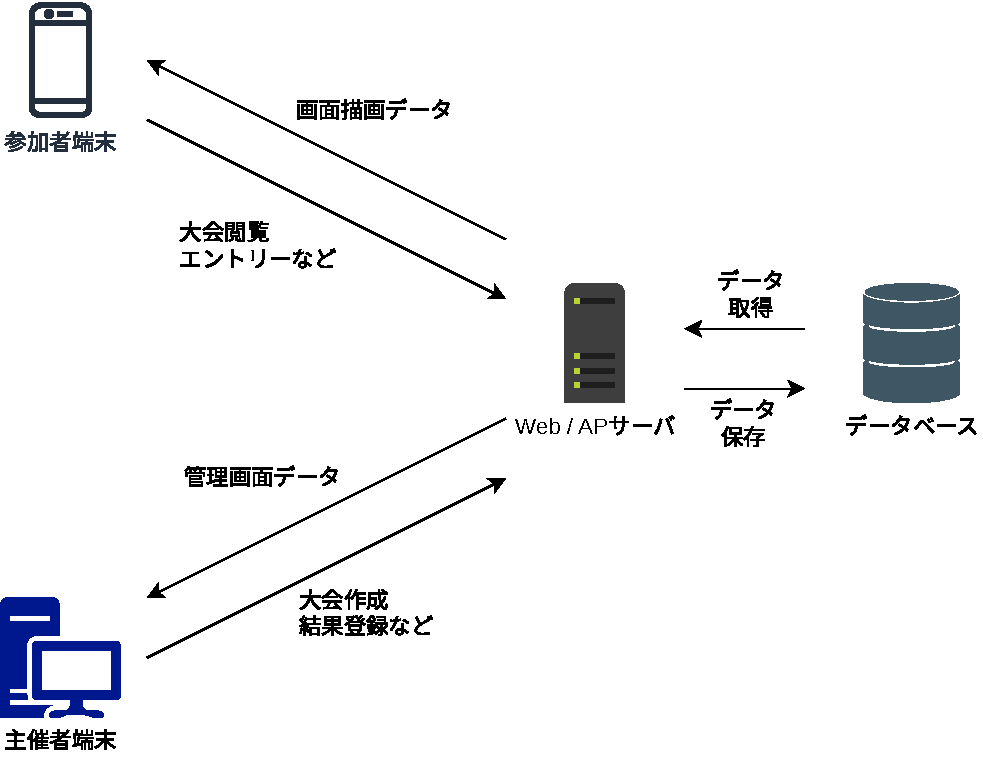
\includegraphics[width=0.85\linewidth]{figures/07/network_design.pdf}
    \caption{ネットワーク構成}
    \label{fig:network_design}
\end{figure}

\subsection{使用サービスおよびミドルウェア仕様}
本システムのネットワーク基盤およびサーバ内で動作する各種サービス、
ソフトウェア・フレームワークの一覧を表~\ref{tab:Services} および表~\ref{tab:Software} に示す。

\begin{table}[H]
    \centering
    \caption{使用するサービス}
    \label{tab:Services}
    \begin{tabularx}{0.85\linewidth}{|X|X|}
        \hline
        \rowcolor{tableblue}
        \multicolumn{1}{|c|}{サービス名} & \multicolumn{1}{c|}{用途} \\ \hline
        Amazon Elastic Compute Cloud (EC2) & Web/AP 統合サーバ \\ \hline
        Amazon Relational Database Service (RDS) & データベースサーバ \\ \hline
    \end{tabularx}
\end{table}

\begin{table}[H]
    \centering
    \caption{使用するソフトウェア・フレームワーク}
    \label{tab:Software}
    \begin{tabularx}{0.85\linewidth}{|X|X|}
        \hline
        \rowcolor{tableblue}
        \multicolumn{1}{|c|}{ソフトウェア・フレームワーク} & \multicolumn{1}{c|}{用途} \\ \hline
        Nginx & Web サーバ（リバースプロキシ） \\ \hline
        Django & Web アプリケーションフレームワーク（APサーバ） \\ \hline
        MySQL & データベース管理システム（DBMS） \\ \hline
    \end{tabularx}
\end{table}